\documentclass[12pt,a4paper]{report}

% --- Packages de base ---
\usepackage[utf8]{inputenc}
\usepackage[T1]{fontenc}
\usepackage[french]{babel}
\usepackage{graphicx}
\usepackage{geometry}
\geometry{hmargin=2.5cm,vmargin=2.5cm}
\usepackage{hyperref}
\usepackage{titlesec}
\usepackage{listings}
\usepackage{xcolor}
\usepackage{amsmath}
\usepackage{array}

% --- Configuration du code source ---
\lstset{
    language=Python,
    basicstyle=\ttfamily\small,
    keywordstyle=\color{blue},
    stringstyle=\color{red},
    commentstyle=\color{green!60!black},
    breaklines=true,
    numbers=left,
    numberstyle=\tiny,
    frame=single
}

% --- Informations du document ---
\title{Rapport de Projet M1 IA \\ Classification de Séries Temporelles pour la Supervision Système}
\author{Projet M1 IA}
\date{\today}

\begin{document}

\maketitle

\tableofcontents

\chapter{Introduction}

Ce projet s'inscrit dans le cadre du module d'intelligence artificielle en Master 1. L'objectif est de classer des séries temporelles issues de la supervision de systèmes informatiques. Ces données représentent l'activité de composants essentiels comme le processeur (CPU), le disque et la mémoire vive (RAM).

L'enjeu est de pouvoir identifier automatiquement le type d'activité à partir de traces d'exécution. Dans un contexte réel, cela permettrait de surveiller l'état de santé d'un serveur ou d'identifier des comportements anormaux.

\section{Objectifs du projet}
Le travail demandé consiste à tester et comparer trois approches différentes :
\begin{itemize}
    \item Les réseaux de neurones récurrents de type LSTM.
    \item Les réseaux de neurones convolutionnels (CNN 1D).
    \item Les modèles plus récents basés sur le mécanisme d'attention (Transformers).
\end{itemize}

\chapter{Présentation et préparation des données}

\section{Origine des données}
Les données utilisées proviennent d'un dépôt public regroupant des traces d'exécutions d'outils de tests de charge. Chaque échantillon est un fichier CSV contenant plusieurs colonnes de mesures système prises à intervalles réguliers.

\section{Exploration visuelle}
Avant de traiter les données, nous avons visualisé les signatures caractéristiques de chaque catégorie. Par exemple, une activité CPU intense se traduit par une charge élevée et constante sur le processeur, tandis qu'une activité disque montre des pics lors des phases de lecture ou d'écriture.

\begin{figure}[h]
    \centering
    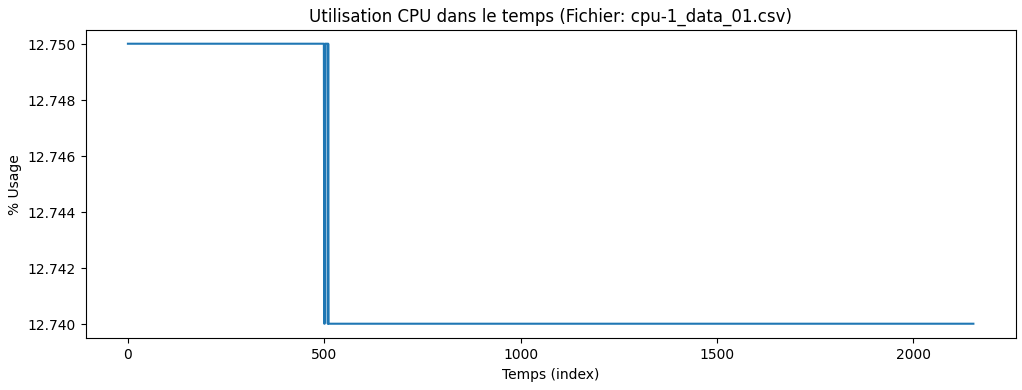
\includegraphics[width=0.8\textwidth]{capture/PremiereVisualisation.png}
    \caption{Visualisation initiale d'une trace système}
    \label{fig:visu_initiale}
\end{figure}

\begin{figure}[h]
    \centering
    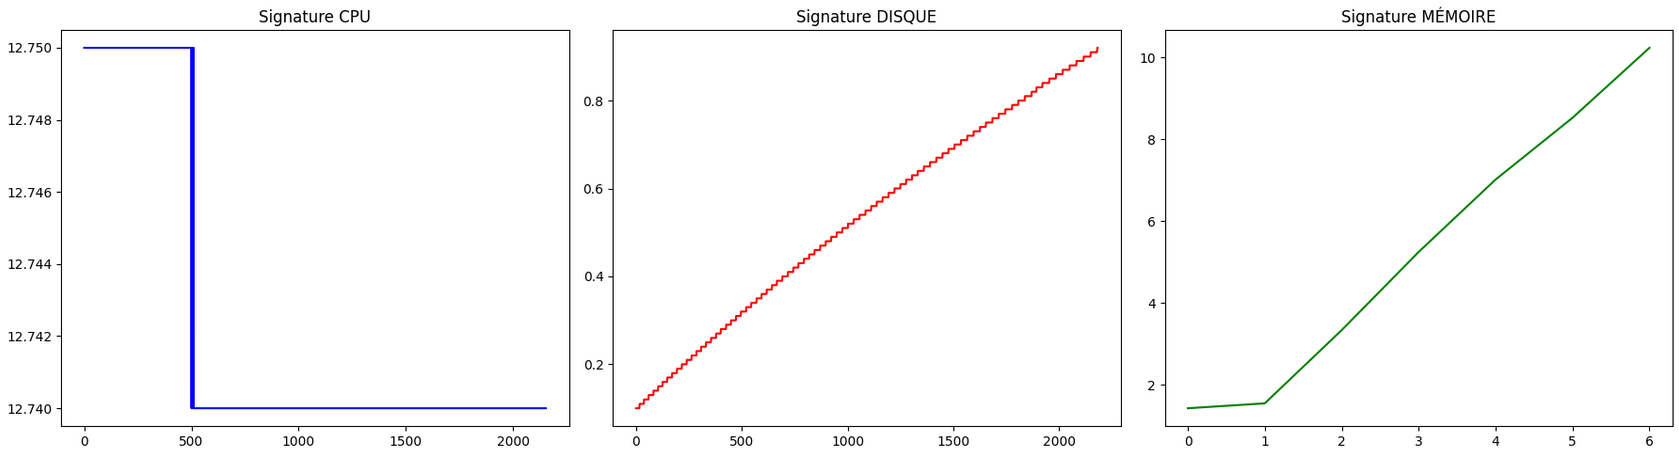
\includegraphics[width=1\textwidth]{capture/ComparaisonSignature.png}
    \caption{Comparaison des signatures CPU, Disque et Mémoire}
    \label{fig:signatures}
\end{figure}

\section{Prétraitement}
Pour que les modèles puissent apprendre efficacement, les données subissent plusieurs transformations :
\begin{itemize}
    \item \textbf{Sélection des colonnes} : Nous retenons l'usage global du CPU, l'occupation de la RAM et les taux de lecture/écriture disque.
    \item \textbf{Normalisation} : Les valeurs sont ramenées entre 0 et 1 pour éviter que les grandes unités (comme les octets de mémoire) n'écrasent les petites (pourcentages CPU).
    \item \textbf{Fenêtrage} : Les données sont découpées en séquences de 50 unités de temps. C'est ce bloc de 50 points qui sera donné en entrée aux modèles.
\end{itemize}

\end{document}
